\documentclass[reprint, amsmath, amssymb, aps]{revtex4-2}

\usepackage{graphicx}% Include figure files
\usepackage{dcolumn}% Align table columns on decimal point
\usepackage{bm}% bold math
\usepackage{hyperref}% add hypertext capabilities
\usepackage[font=scriptsize,labelfont=bf, justification=justified]{caption}% change fontsize in captions
\usepackage{float}
\usepackage{booktabs}% cool table style
\hypersetup{
	colorlinks=true,       % false: boxed links; true: colored links
	linkcolor=black,        % color of internal links
	citecolor=black,        % color of links to bibliography
	filecolor=black,     % color of file links
	urlcolor=black         
}

\begin{document}
	
\title{PHYC30170 Physics with Astronomy and Space Science Lab 1;\\The Brusselator - A Computational Example of Chemical Oscillations}

\author{Daragh Hollman}
\email{daragh.hollman@ucdconnect.ie}
\date{\today}

\begin{abstract}
This is the abstract...
\end{abstract}

\maketitle

\section{Introduction}

What are chemical oscillations and what are their modern applications.\\

What is the Brusselator?

\subsection{Oscillations in a Chemical System}

Talk about the origins of chemical oscillations. Boris Belousov. The beliefs of the scientific community at the time that oscillations in a chemical system couldn't exist due to the laws of thermodynamics.

\subsection{Chemical Equations}

Discuss how chemical equations work and how you can get rate equations from these. Describe how this can be broken down into differential equations.

\subsection{The Brusselator}

Discribe the specific brussellator system and the rate equations involved. Describe the break down into two first order ODEs. Define the species of interest and discuss how they are autocatylitic.\\

The chemical equations of the Brusselator are described in the lab manual as follows \cite{manual}:
\begin{align}
	\begin{aligned}
	A &\rightarrow X & (a)\\
	B + X &\rightarrow Y + D & (b)\\
	2X + Y &\rightarrow 3X & (c)\\
	X &\rightarrow C & (d)
	\end{aligned}
\end{align}

With ODEs given by:
\begin{align}
	\begin{aligned}
	\frac{dX}{dt} &= A - (B + 1)X + X^2 Y & (a)\\
	\frac{dY}{dt} &= BX - X^2 Y & (b)
	\end{aligned}
\end{align}


Describe the stable position of the system and derive it.\\

At any stable point, the rate of change of $X$ and $Y$ is zero.
\begin{equation}
	\frac{dX}{dt}=0\,\text{  ;  }\frac{dY}{dt}=0
\end{equation}Hence,


Discuss what will be looked at, i.e. phase space diagrams and concentration evolutions. The variation of intial conditions and the fixed constants etc.\\

\section{Computational Methods}

\subsection{The Euler Method}

\subsubsection{The Application of the Euler method to the System}

\subsection{Error Analysis of the Euler Method}

\section{Results and Discussion}

\subsection{Varying the initial conditions}

\begin{figure*}
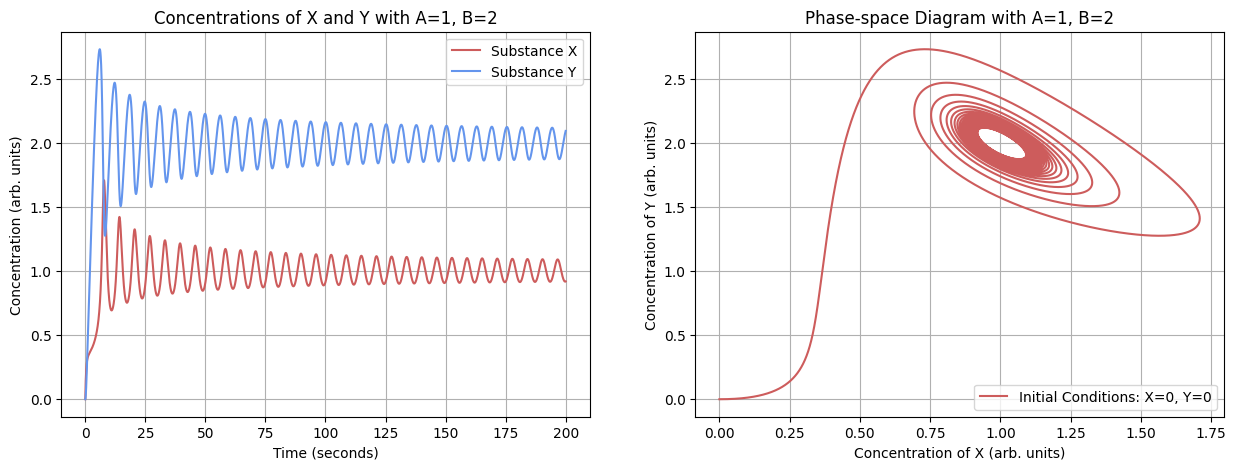
\includegraphics[width=2\columnwidth]{combinedPlot.png}
\caption{\label{fig:combinedPlot}Example caption}
\end{figure*}

\begin{figure*}
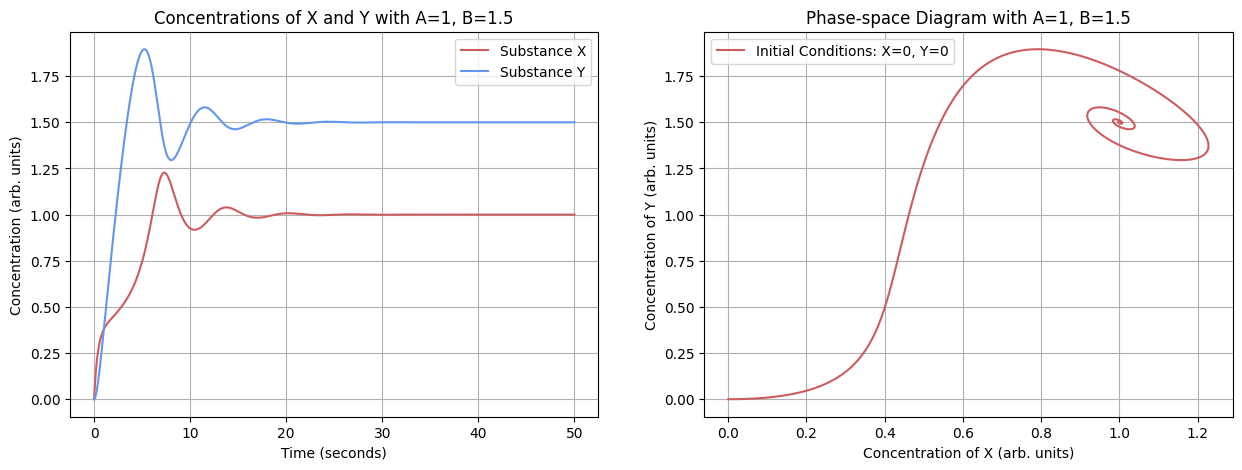
\includegraphics[width=2\columnwidth]{combinedPlot_fallToStable.png}
\caption{\label{fig:combinedPlot}Falls to stable point}
\end{figure*}

\begin{figure}
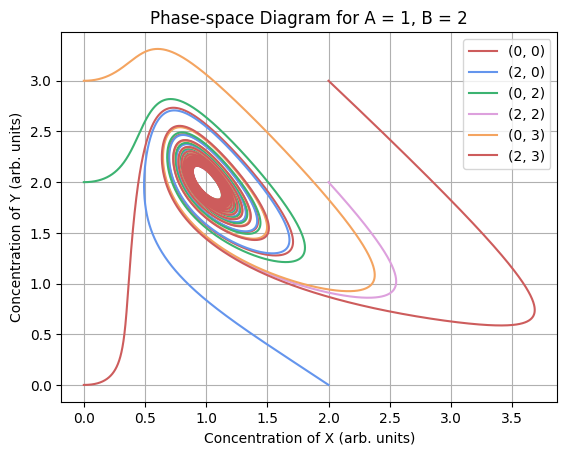
\includegraphics[width=0.85\columnwidth]{variationOfInitialConditions_phase.png}
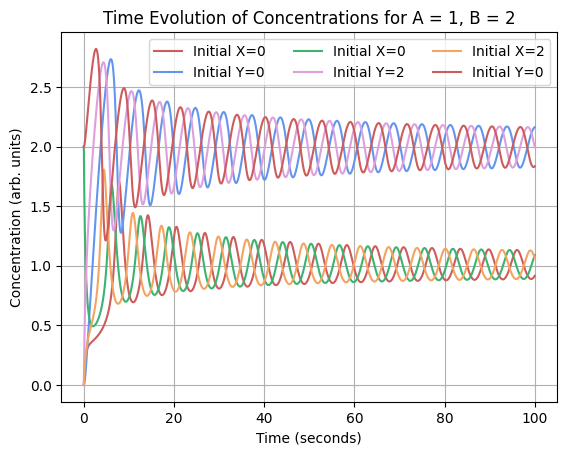
\includegraphics[width=0.85\columnwidth]{variationOfInitialConditions_evolution.png}
\caption{\label{fig:combinedPlot}Variation of initial conditions}
\end{figure}

\section{Conclusion}

\clearpage
\bibliography{chemOscillationsReferences.bib}

\end{document}



